%% Copernicus Publications Manuscript Preparation Template for LaTeX Submissions
%% ---------------------------------
%% This template should be used for copernicus.cls
%% The class file and some style files are bundled in the Copernicus Latex Package, which can be downloaded from the different journal webpages.
%% For further assistance please contact Copernicus Publications at: production@copernicus.org
%% https://publications.copernicus.org/for_authors/manuscript_preparation.html


%% Please use the following documentclass and journal abbreviations for preprints and final revised papers.

%% 2-column papers and preprints
\documentclass[gmd, manuscript]{copernicus}



%% Journal abbreviations (please use the same for preprints and final revised papers)


% Advances in Geosciences (adgeo)
% Advances in Radio Science (ars)
% Advances in Science and Research (asr)
% Advances in Statistical Climatology, Meteorology and Oceanography (ascmo)
% Annales Geophysicae (angeo)
% Archives Animal Breeding (aab)
% ASTRA Proceedings (ap)
% Atmospheric Chemistry and Physics (acp)
% Atmospheric Measurement Techniques (amt)
% Biogeosciences (bg)
% Climate of the Past (cp)
% DEUQUA Special Publications (deuquasp)
% Drinking Water Engineering and Science (dwes)
% Earth Surface Dynamics (esurf)
% Earth System Dynamics (esd)
% Earth System Science Data (essd)
% E&G Quaternary Science Journal (egqsj)
% European Journal of Mineralogy (ejm)
% Fossil Record (fr)
% Geochronology (gchron)
% Geographica Helvetica (gh)
% Geoscience Communication (gc)
% Geoscientific Instrumentation, Methods and Data Systems (gi)
% Geoscientific Model Development (gmd)
% History of Geo- and Space Sciences (hgss)
% Hydrology and Earth System Sciences (hess)
% Journal of Bone and Joint Infection (jbji)
% Journal of Micropalaeontology (jm)
% Journal of Sensors and Sensor Systems (jsss)
% Magnetic Resonance (mr)
% Mechanical Sciences (ms)
% Natural Hazards and Earth System Sciences (nhess)
% Nonlinear Processes in Geophysics (npg)
% Ocean Science (os)
% Polarforschung - Journal of the German Society for Polar Research (polf)
% Primate Biology (pb)
% Proceedings of the International Association of Hydrological Sciences (piahs)
% Scientific Drilling (sd)
% SOIL (soil)
% Solid Earth (se)
% The Cryosphere (tc)
% Weather and Climate Dynamics (wcd)
% Web Ecology (we)
% Wind Energy Science (wes)


%% \usepackage commands included in the copernicus.cls:
%\usepackage[german, english]{babel}
%\usepackage{tabularx}
%\usepackage{cancel}
%\usepackage{multirow}
%\usepackage{supertabular}
%\usepackage{algorithmic}
%\usepackage{algorithm}
%\usepackage{amsthm}
%\usepackage{float}
%\usepackage{subfig}
%\usepackage{rotating}


\begin{document}

\title{Constraining the carbon cycle in JULES-ES-1.0}

% \Author[affil]{given_name}{surname}

\Author[1,2]{Doug}{McNeall}
\Author[1]{Eddy}{Robertson}
\Author[1,2]{Andy}{Wiltshire}

\affil[1]{Met Office, FitzRoy Road, Exeter, EX1 3PB}
\affil[2]{College of Engineering, Mathematics, and Physical Sciences, University of Exeter, Exeter, EX4 4QE, UK}
\affil[3]{College of Life and Environmental Sciences, University of Exeter, Exeter, EX4 4RJ, UK}

%% The [] brackets identify the author with the corresponding affiliation. 1, 2, 3, etc. should be inserted.

%% If an author is deceased, please mark the respective author name(s) with a dagger, e.g. "\Author[2,$\dag$]{Anton}{Aman}", and add a further "\affil[$\dag$]{deceased, 1 July 2019}".

%% If authors contributed equally, please mark the respective author names with an asterisk, e.g. "\Author[2,*]{Anton}{Aman}" and "\Author[3,*]{Bradley}{Bman}" and add a further affiliation: "\affil[*]{These authors contributed equally to this work.}".


\correspondence{Doug McNeall (doug.mcneall@metoffice.gov.uk)}

\runningtitle{Constraining the historic carbon cycle in JULES-ES1.0}

\runningauthor{McNeall et al.}





\received{}
\pubdiscuss{} %% only important for two-stage journals
\revised{}
\accepted{}
\published{}

%% These dates will be inserted by Copernicus Publications during the typesetting process.


\firstpage{1}

\maketitle

\begin{abstract}

Land surface models are an important tool in the study of climate change and its impacts, but their use can be hampered by uncertainties in the differences between the models and the real world. Uncertainty quantification (UQ) methods have been developed in order to quantify those differences, how to minimise them, and how to asses their impact on the use of models in policy advice. In this study we use UQ methods to constrain a large ensemble of JULES-ES-1.0 using modern observations of the carbon cycle. We provide information to modellers about the sensitivity of model outputs to changes in uncertain inputs, and identify a model discrepancy which is difficult to remove by tuning those uncertain inputs. We explore the resulting constraint on the behaviour of the carbon cycle during the historical period.

As the land surface model is computationally expensive, we use a statistical proxy, termed an emulator, trained on a carefully selected perturbed parameter ensemble of model runs, driven by a historical climate reanalysis . We take an "iterated refocussing", or "History Matching" approach to constraining JULES, first running an initial ensemble and training the emulator, before using it to choose a second wave of ensemble members consistent with historical land surface observations and expectations.

We provide an ensemble of JULES runs that are statistically consistent with past land surface behaviour, and an associated constraint of the joint distribution of input parameters. We show that an emulator is a useful tool for providing modellers and policymakers information about the nature of the Earth system configuration of the land surface model JULES.

\end{abstract}

\copyrightstatement{TEXT} %% This section is optional and can be used for copyright transfers.

\section{Analysis plan}

\subsection{\textcolor{red}{AJW Notes}}
\textcolor{red}{A few thoughts on this paper following our previous discussions. This paper describes the ensemble, the available data and the emulator? The ensemble is focused on the terrestrial carbon sink. The next paper focuses on constraining the historical C sink and possibly a third looks at the carbon feedback terms.}

\textcolor{red}{This paper therefore presents the original 500 members of wave 1, followed by the 500 of wave 2. wave 2 by design is broad but less broad than 1 aimed a filling a tighter parameter space, but importantly is a plausible set of experiments from which further work can be developed. wave 2 should therefore be compared to CMIP and TRENDY simulations. We also learn alot about our model and its sensitivities using the analyses presented which is a result in itself and gives us a decent emulator to use going forward}



------

Our guiding principles for this paper: what does comparing the model output with observations tell us about where to run the model, and also about the history of the carbon cycle?

Analyses
\begin{enumerate}
    \item Introduction, motivation and JULES context
    \item Run failures
    \item History matching and constraint
    \item Sensitivity analysis
    \item Discrepancy hunting
\end{enumerate}

Supplementary or in development

\begin{enumerate}
    \item Emulator performance
    \item Comparison with other ensembles
    \item History matching
    \item Sensitivity analysis
    \item Discrepancy hunting
\end{enumerate}

An extension to consider: what happens when we project the constrained space forwards through time. For this, we need runs using future boundary conditions.

\introduction  %% \introduction[modified heading if necessary]

\begin{enumerate}
    \item Jules version, aims, context 
    \item Uncertainty Quantification for model development
\end{enumerate}

Land surface models are an important tool in the study of climate change and its impacts, but their use can be hampered by uncertainties in the differences between the models and the real world. Uncertainty quantification (UQ) methods have been developed in order to quantify those differences, how to minimise them, and how to asses their impact on the use of models in policy advice.

We'd like to constrain the uncertain input parameters using data.
We'd like to know which parameters are important for which outputs.
We'd like information on model discrepancy. Is there a "best" configuration.
We'd like and ensemble which can be used for impacts/future projections. Covering reasonable uncertainty.


Top-down approach, compared to bottom-up approach of e.g Baker et al.

We run Jules-ES-1.0 in a 500-member ensemble, driven by historical reanalysis. Each ensemble member has a different configuration of 32 input parameters, identified as potentially important in influencing land surface dynamics important by the model developers (see table /ref{table:parameters}.

* Table of input parameter descriptions*
%t
\begin{table*}[t]
\caption{Uncertain input parameters in JULES-ES-1p0}
\label{table:Parameters}
\begin{tabular}{l r}
\tophline
Parameter & Description  \\ 
\middlehline

alpha\_io & Quantum efficiency (mol CO2 per mol PAR photons). \\ 
  lai\_max\_io & Maximum LAI. \\ 
  b\_wl\_io & Allometric exponent relating the target woody biomass to the leaf area index.\\ 
  fd\_io & Scale factor for dark respiration.\\ 
  g\_area\_io &  Disturbance rate (/360days).\\ 
  n\_inorg\_turnover &Parameter controlling the lifetime of the inorganic N pool. \\ 
  r\_grow\_io & Growth respiration fraction.\\ 
  lma\_io & Leaf mass per unit area (kgLeaf m-2). \\ 
  a\_wl\_io & Allometric coefficient relating the target woody biomass to the leaf area index (kg carbon m-2). \\ 
  bio\_hum\_cn &  Parameter controlling ratio of C to N for BIO and HUM pools.\\ 
  nmass\_io &  Top leaf nitrogen content per unit mass (kgN kgLeaf-1).\\ 
  kaps\_roth &  Specific soil respiration rate for the RothC submodel for each soil carbon pool.\\ 
  hw\_sw\_io & Ratio of N stem to N heartwood (kgN/kgN) from the TRY database. \\ 
  tleaf\_of\_io & Temperature below which leaves are dropped (K).\\ 
  dqcrit\_io & Critical humidity deficit (kg H2O per kg air). \\ 
  lai\_min\_io & Minimum LAI. \\ 
  tupp\_io & Upper temperature for photosynthesis (deg C). \\ 
  retran\_l\_io & Fraction of retranslocated leaf N.\\ 
  rootd\_ft\_io & Parameter determining the root depth (m). \\ 
  l\_vg\_soil & Switch for van Genuchten soil hydraulic model. \\ 
  dz0v\_dh\_io & Rate of change of vegetation roughness length for momentum with height. \\ 
  f0\_io & CI / CA for DQ = 0. \\ 
  sigl\_io & Specific density of leaf carbon (kg C/m2 leaf).\\ 
  g\_root\_io & Turnover rate for root biomass (/360days). \\ 
  gs\_nvg\_io & Surface conductance (m s-1). \\ 
  retran\_r\_io & Fraction of retranslocated root N.\\ 
  g\_wood\_io &  Turnover rate for woody biomass (/360days).\\ 
  nr\_io &  Root nitrogen concentration (kgN/kgC).\\ 
  knl\_io & Parameter for decay of nitrogen through the canopy, as a function of LAI.\\ 
  sorp & Parameter controlling the leaching of inorganic N through the soil profile. \\ 
  dcatch\_dlai\_io &Rate of change of canopy capacity with LAI (kg m-2).  \\ 
  tlow\_io & Lower temperature for photosynthesis (deg C).\\  
\bottomhline
\end{tabular}
\belowtable{} % Table Footnotes

\end{table*}

The parameters were perturbed randomly, in a Latin hypercube configuration, and within ranges defined by the model developers as being likely to at least produce output from the model.

We identify model variants, and their associated input configurations, where the model produces output that is consistent - within uncertain limits - with modern observations of the carbon cycle. We build statistical models of the relationship between the input configuration and the modern model output - termed emulators - which allow us to visualise and explore these relationships as if we had a much larger ensemble.

Using the ensemble and the emulators, we are able to generate a number of analyses that inform us of the drivers of model behaviour, and the source of model biases and errors. We provide a failure analysis, which allows us to identify parameter setting which cause failure of the model to run. We perform sensitivity analysis, which helps us quantify the effect of perturbing parameters on the model output.

Finding model outputs which match modern observations, we identify parts of input parameter space where the model output is acceptably good. We can rule out parameter settings where the output is not plausible. Constraining using each output in turn allows us to see which outputs are useful for constraining particular inputs. We see relationships between outputs manifest as joint constraint: when one output is used to constrain inputs, this induces a constraint on other, related outputs.

Having constrained both input parameter space and model outputs using modern observations of the carbon cycle, we examine the impact of the modelled carbon budget through time. What is the potential for constraining the carbon budget using only modern observations? What happens if we extend those observations back through time?

Our analysis informs the construction a new ensemble design, with ensemble members picked to lie within the input space not ruled out by a comparison of the model behaviour with modern observations. 

Our aim was to run an iterated experiment to create an ensemble of JULES runs that would allow  a number of different types of analysis. Our objectives were 1) to find an ensemble of JULES runs that would represent (and span) uncertainty in both model input parameters and historical land surface behaviour, thus creating a basis ensemble for a UQ analysis of past behaviour and future projections. 2) Explore if some uncertain input parameters could be constrained by comparison of the model outputs with observational data and 3) To create an ensemble that could be used for sensitivity analyses, identifying the most important inputs. 

All of these objectives are well served by creating an ensemble that allows surrogate models, or emulators, to be trained and used in place of the full simulator.

Many climate model experiments have only a limited amount of computational budget, and modellers must decide how to spend that budget. While JULES-ES-1p0 is relatively cheap, and in practice we were not constrained (within reason) by computational budget, we decided to mimic a full climate model experiment. Such an experiment might have access to a few tens to a few thousand model runs. We decided to run the experiment with approximately 1000 runs, somewhere near the middle of this range.

Our experiment was inspired by the history matching procedure, otherwise known as "iterated refocussing", in which an initial ensemble is run, ensemble members (and the associated input space) deemed too far from reality are ruled out, and a further wave of ensemble members are run in the input space that has not been ruled out yet. At each stage, a surrogate model, or emulator is trained on the model outputs, predicting model output at inputs not yet run. This emulator is used to predict which inputs will not be ruled out in the next wave, and for new design points to be selected from these candidates. The emulator should become more accurate in the valid input space at each wave. As this was an exploratory design process, we did not attempt to optimise this process by selecting an ideal number of runs for each stage, but instead chose reasonable numbers, before deciding to go further if necessary.

\section{Constraining the historical carbon cycle}

Our experiment has a "top-down" structure, in that we attempt to constrain input parameter space (and therefore model behaviour) by comparison to observational data, starting from a global overview. We use very little prior information to choose initial input parameter ranges, we run the model globally, and we compare globally averaged model output to globally averaged observations, starting with a few important properties, and working towards more detail. An alternative experiment structure might be classed as "bottom up" - starting with standard parameters and working away from them, focusing on individual processes within the model, and comparing with much more focused model output and observations, both in time and in space. Ultimately, both of these types of experiment will be important in integrating new processes into larger models in a model development process.

We set the budget for the initial exploratory ensemble to 500 members, a little over 10 members per input parameter recommended as a rule of thumb by (cite). 

The aim of the initial ensemble was to explore the limits of parameter space, and ensure that any future constrained ensemble would be interpolating and not extrapolating from the initial design. For that reason, we implored the model developers to set ranges on the parameter perturbations to be as wide as possible, while still having a good chance of running and at least providing output.

We elicited reasonable multiplication factors from the modeller (Wiltshire), based on the uncertainty of each parameter, and an estimate of the limits of the parameters at which the model would even run. The multiplication factors were perturbed in a space filling design, in order to best cover input space and help build Gaussian process emulators, which can have problems if design points are spaced too closely. We chose a maximim Latin Hypercube design using the R package LHS (*cite*). The design chosed was the Latin hypercube with the largest minimum distance, from a set of 10,000 generated candidates.

The initial ensemble (designated wave00) started with 500 members, each with a different setting of 32 uncertain parameters. Many of these parameters have different values for the 13 different plant functional types (PFTs) in JULES. If each of these were perturbed independently, there would potentially be an intolerably large input space. To combat this explosion of dimensions, we decided to perturb each of the PFTs together, by a multiplication factor for each parameter. This choice was computationally convenient for a top-down, globally averaged experiment, but we see great potential for optimising the values of these parameters for individual PFTs in further work. 

\begin{figure*}[t]
\includegraphics[width=12cm]{./graphics/lhs_range.pdf}
\caption{Parameter multiplication factor ranges the ensemble design.}
\label{fig:lhs_range}
\end{figure*}

\subsection{Failure analysis}\label{ssec:failure-analysis}

We analyse the ensemble to remove "failed" runs, and remove ensemble members in parts of parameter space that cannot hope to produce a useful simulation of the carbon cycle. First, we map ensemble members where the model crashed or failed to run, perhaps due to numerical error (termed "failed"). Second, we identify parts of parameter space where important parts of the carbon cycle are completely missing - that is, basic carbon cycle quantities are at or close to zero at the end of the run (termed "zero carbon cycle"). For this second class, we choose a threshold of mean modern global NPP close to zero (* scale data to find out)

The nature of perturbed parameter ensembles is that there is often a setting of some parameters that makes up for a poor choice of a particular parameter, and so outright and easily identifiable thresholds for failure in the marginal range of a particular parameter are rare. However, careful visualisation and analysis can give the modeller a good idea of regions of parameter space that can be removed, or parameters that the model is particularly sensitive to.

in fig. \ref{fig:run-failure-pairs}, we see a pairs plot of "failed" runs (upper right panels) and, "zero carbon cycle" panels (lower left panels). The plot shows the two-dimensional projections of run failures against each pair of inputs, allowing visual identification of inputs that control failures, and any potential two-way interactions.

For example, we can see that both $f0\_io$ and $b\_wl\_io$ have important thresholds, beyond which there is almost no chance of a functioning carbon cycle. As there appears little to no interaction between these two, this presents as a nearly-blank plot at the intersection of the parameters on the plot, with inputs identifying zero-carbon runs around the edges of the sub plot.

\begin{figure*}[t]
\includegraphics[width=12cm]{./graphics/run-failure-pairs.pdf}
\caption{Pairs plot of the locations in (normalised) input space of the ensemble members that did not run/failed.}
\label{fig:run-failure-pairs}
\end{figure*}

\begin{figure*}[t]
\includegraphics[width=12cm]{./graphics/run-failure-hists.pdf}
\caption{Histograms of the locations in (normalised) input space of the ensemble members that did not run/failed.}
\end{figure*}


\subsection{Initial direct constraints}

Our "iterated refocussing" experiment use a combination of formal and informal methods to sequentially constrain input parameter space and model behaviour, dependent on both expertise and expectation of the modeller, and more formal comparison with observational data.

We therefore use a number of "waves" of ensemble runs, and  "levels of constraint", where those waves are compared with data, or modified by the modeller. 

Our aim for the initial ensemble is primarily to train a good surrogate model (here a Gaussian process emulator), and therefore we require relatively smooth output across the inputs space, without discontinuities or highly nonlinear and poor behaviour that might bias an emulator.

Our initial (wave00) ensemble of 499 members is sequentially constrained; to "Level0" by removing 24 ensemble members which do not run (see section \ref{ssec:failure-analysis}, to "Level 1" by removing the 50 remaining ensemble member outside of the threshold in $F0$ identified in that section, and "Level 1a" by removing the 64 remaining members outside the threshold in $B\_WL\_IO$. This leaves us with a "level 1a" ensemble of 361 members that at least run and have a minimally functioning carbon cycle.

\subsubsection{minimally constrained ensemble behaviours}

The globally averaged carbon cycle and land surface behaviour of the minimally ensemble (level 1a) can be seen in fig. \ref{fig:carbon-cycle-timeseries-waves-constrained}, and anomalies compared to the average of the first 20 years of the runs can be seen in fig. \ref{fig:carbon-cycle-timeseries-anomaly-waves-constrained}, in the blue lines.

The ensemble displays a very wide range of both absolute levels and changes in a selection of carbon cycle and land surface properties, compared to the model run at standard settings (black). For example, NPP runs from approximately zero to over 150 GtC/year. Soil carbon stocks are between zero and more than 4000 GtC, and Vegetation stocks range from 0 to over 2000 GtC.

A large number of ensemble members have a hugely diminished carbon cycle and carbon cycle stocks compared to the standard member. This can be seen from examining the histograms of the modern values of a number of key carbon cycle properties in fig. \ref{fig:wave00-level1a-modern-value-hists}, compared to the values of the standard member (vertical lines).

In particular, most ensemble members have a very low tree fraction, and a higher bare soil fraction than the standard member - It seems particularly easy to kill global forests when perturbing parameters. Vegetation and soil carbon levels are very low. 

[Note: this brings into question whether a top-down UQ method is advisable for JULES. Or ware we just perturbing too much? ]

[Note: A number of TS show large deviations from reality - discarded.]

In many indicators, perturbing parameters affects the overall level of the carbon cycle property, with it's behaviour through time being only a secondary source of variance at, say, the end of the model run. That is, the carbon cycle level at the end of the run is more closely related to its level at the beginning of the run than it is to its change over time. Having said that, there is variability in the behaviour of the carbon cycle over time, as can be seen in fig. \ref{fig:carbon-cycle-timeseries-anomaly-waves-constrained}. Here, we examine a selection of the most important indicators, and examine their change in behaviour over time, or anomaly from the starting value. We see for example, that changing the parameters can make soil and vegetation carbon increase or decrease over the simulated century and a half of the model run. 


\subsection{Level 2 Constraints}

We can constrain both the historical behaviour of the model and the model parameter input space by comparison of the model behaviour with observations and other model simulations.
The simplest way to constrain the historical behaviour of the carbon cycle is by removing from the ensemble model runs that lead to implausible values of basic carbon cycle quantities in the modern era. These constraints are outlined in table \ref{table:level_2_constraints}.

Our strategy is to exclude model variants that have soil or vegetation carbon stocks, net primary production (NPP) or net biome production (NBP) in the modern era that are inconsistent with modern observations or understanding. This approach borrows from the more formal process of history matching, in that ensemble members deemed implausible are excluded. In history matching, a formal statistical process is used, whereas in this first section, we are concerned with simply removing a number of very poorly behaving model variants, such that the modeller is certain that they don't offer useful information about the carbon cycle.

A challenge when comparing models of the land surface with the carbon cycle is the lack of model-independent observations back through time, and the relatively large uncertainty in comparing the model dynamics with the true behaviour of the system. Because of this, it is important to be tolerant to a wide range of behaviours in the model itself. 

In a "tolerance to error" approach, the modeller (Wiltshire) gave estimated ranges for Vegetation and Soil carbon stocks, NBP and NPP at the end of the model run (2013), with instruction to be conservative - that is with enough range to be sure to encompass any reasonable uncertainties (see table \ref{table:level_2_constraints}). These ranges were considerably wider than the ranges given by the AR5, for example.

Because of this wide tolerance of modern behaviours, we perhaps should not be too optimistic that large regions of input space, or potential histories of the carbon cycle, should be excluded (alternatively that the space of possible histories and input space should be overly constrained).

However, even given the wide ranges of tolerable behaviour, a large number of our ensemble members are excluded. Of the 361 ensemble members that run, and have non-zero carbon cycle properties (constraint level 1a), only 37 (10.2\%) fall within the wide bounds set by the modeller Wiltshire.

%% TWO-COLUMN TABLE
%%% The different columns must be seperated with a & command and should
%%% end with \\ to identify the column brake.

%t
\begin{table*}[t]
\caption{Levels of constraint}
\label{table:levels_of_constraint}
\begin{tabular}{l r}
\tophline
Level & Constraint  \\ 
\middlehline
Level 0  & Model Runs \\
Level 1 & $F0 < 0.9$ \\
Level 1a & $B\_WL\_IO > 0.15 $ \\ 
Level 2  & NPP, NBP, cVeg and cSoil \\

\bottomhline
\end{tabular}
\belowtable{} % Table Footnotes

\end{table*}

%t
\begin{table*}[t]
\caption{Level 2 output constraints}
\label{table:level_2_constraints}
\begin{tabular}{l r r}
\tophline
Constraint & Minimum & Maximum \\ 
\middlehline
NBP & 0 GtC/yr &  10 GtC/yr\\
NPP & 35 GtC/yr & 80 GtC/yr \\
Soil Carbon stock & 750 GtC &  3000 GtC\\ 
Vegetation Carbon stock & 300 GtC & 800 GtC \\

\bottomhline
\end{tabular}
\belowtable{} % Table Footnotes

\end{table*}


%%% TWO-COLUMN FIGURES
%
%%f
\begin{figure*}[t]
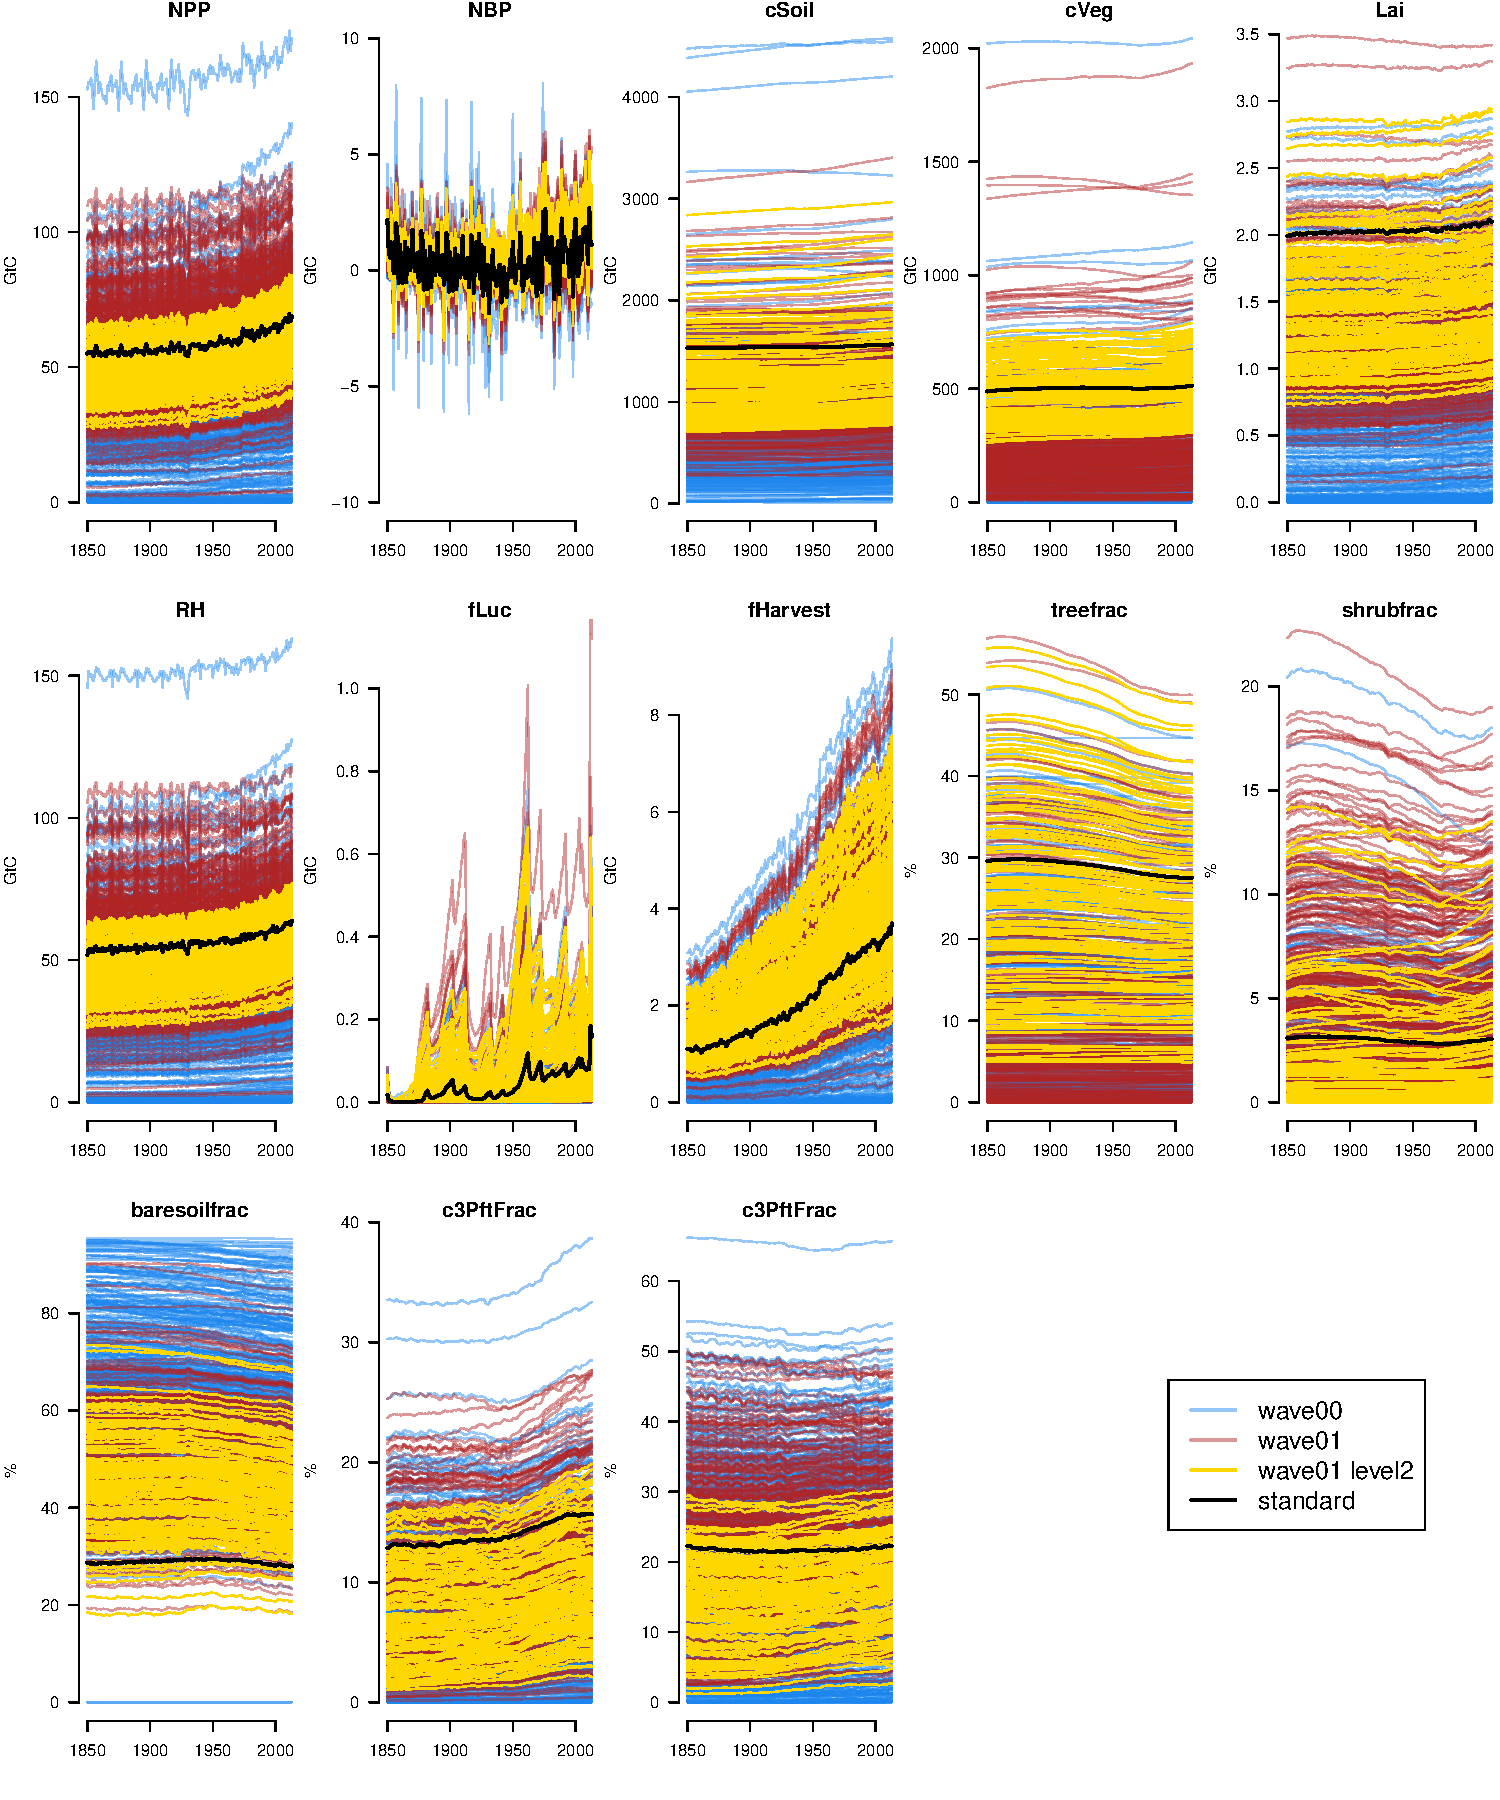
\includegraphics[width=12cm]{./graphics/carbon-cycle-timeseries-waves-constrained.pdf}
\caption{Primary carbon cycle quantities in the JULES ensemble.}
\label{fig:carbon-cycle-timeseries-waves-constrained}
\end{figure*}

%%% TWO-COLUMN FIGURES
%
%%f
\begin{figure*}[t]
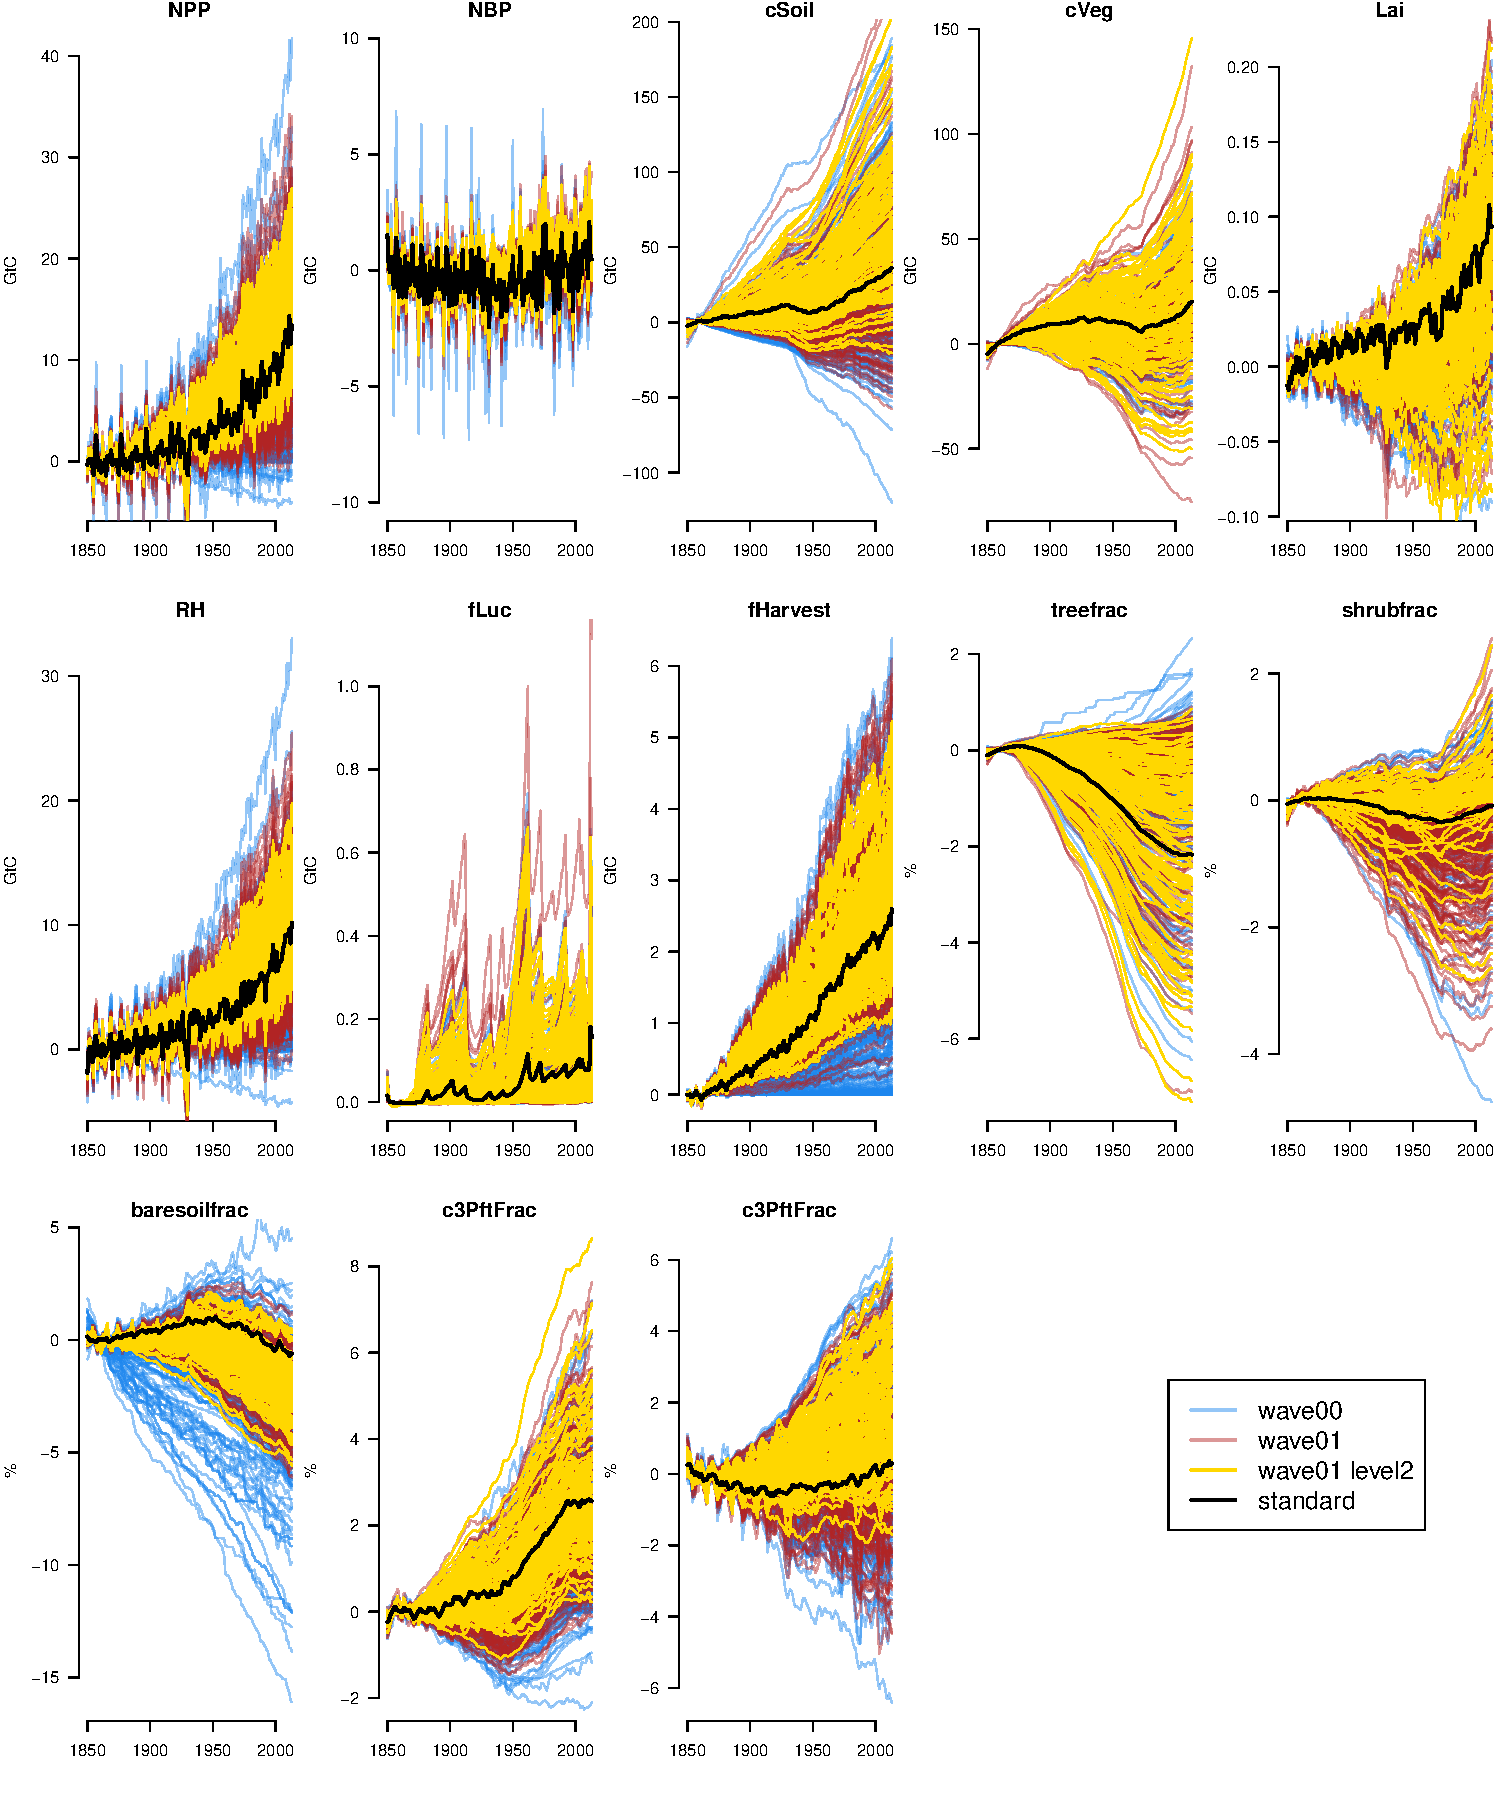
\includegraphics[width=12cm]{./graphics/carbon-cycle-timeseries-anomaly-waves-constrained.pdf}
\caption{Primary carbon cycle anomaly quantities in the JULES ensemble.}
\label{fig:carbon-cycle-timeseries-anomaly-waves-constrained}
\end{figure*}


\begin{figure*}[t]
\includegraphics[width=12cm]{./graphics/level_2_constraints_hists.pdf}
\caption{level 1 constraint histograms}
\label{fig:level_2_constraints_hists}
\end{figure*}


%%% TWO-COLUMN FIGURES
%
%%f
\begin{figure*}[t]
\includegraphics[width=12cm]{./graphics/wave00-level1a-modern-value-hists.pdf}
\caption{Histograms of the modern value of carbon cycle properties in the wave00 ensemble, constrained to level1a (non-running members and zero carbon excluded). [Note fix units on the vectors]}
\label{fig:wave00-level1a-modern-value-hists}
\end{figure*}


\subsection{Design for Second wave (Wave01)}

Only a very small proportion of ensemble members (37) conform to the basic "level 2" constraints expected of a useful model by our modeller. We would like to have a larger number of ensemble members in this range, so that any emulator we build has enough detail to be useful, and we can accurately map out viable input space.

We wish to run more ensemble members within a valid input space, and so we formally history match to the level 2 space, in order to generate an input design for a new wave of ensemble members.

\subsubsection{History matching}

History matching details and equations here.

We history match so that the 95\% range matches the limits given to us by Wiltshire - i.e. the "level 2" constraints. 

We use a Gaussian process emulator to do the history matching.

\subsubsection{Gaussian Process emulators} 

Gaussian Process emulator equations and summary details here.

\subsubsection{Behaviour of second wave}

Constrained, but many ensemble members lie outside of level 2 constraints, due to emulator error, and tolerance to error approach.

\subsubsection{Behaviour of second wave level2}

Ensemble is constrained in many ways, but not in others - quantify and document.

\section{What we need to take the next steps in the analysis}

\begin{itemize}
    \item Modern observations corresponding to model outputs.
    \item Expert-derived limits using above.
    \item CMIP6 boundaries of above.
    \item Model outputs (through time) we'd like to include (regional forest fraction, atmospheric carbon growth, total land carbon).
\end{itemize}

\begin{enumerate}
    \item 
\end{enumerate}


\section{Results}



\section{Sensitivity Analysis}
We use the emulator fit to a range of outputs to perform several types of sensitivity analysis.

\subsection{Global one-at-a-time Sensitivity}

A one-at-a-time (OAAT) sensitivity gives a simple and easy-to-interpret measure of the impact of each input on a variety of outputs, but does not include the effects of any interactions between inputs (for example, a non-linear change in model outputs as two or more inputs vary together).  

A one-at-a-time analysis can be completed with a relatively small number of model runs - for example, a low, middle and high run for each parameter in our 32 input dimension example would take fewer than 100 runs. However, using an emulator allows us to better characterise the response of the model across the entire sweep of each parameter.

We fit a gaussian process emulator (direct km) to each global summary output, both as a ``modern value'' (mean of 1994 - 2014), and as an ``anomaly" (change since 1850-1870).

We sample from the input space in a one-at-a-time fashion: each input is sampled uniformly across it's input space, with all other inputs held at median values. The variance of the mean emulated output as each input is varied is then used as a measure of the sensitivity of that output to the corresponding input. Variance is used as opposed to magnitude of change, as we expect some model outputs not to rise or fall monotonically as an input varies.

Different model outputs are clearly sensitive to different model inputs, and so we also seek ways of summarising sensitivity across model outputs. One method is simply to find the mean effect across model outputs. Sensitivities are normalised so that they lie in a $[0 -1]$ range for each output. Summary measures for each input are then averaged across all outputs, and the plotted inputs are ranked by their average influence across all outputs. Individual sensitivities and summaries can be seen in fig. \ref{fig:oat_var_sensmat_level1a_Y} for the modern value, and in fig. \ref{fig:oat_var_sensmat_level1a_YAnom} for the change over the historic period of the ensemble. 

\subsection{FAST sensitivity analysis}

We use Fourier Amplitiude Sensitivity Test (FAST) as a further measure of global sensitivity of the model outputs to its inputs. The test is administered as the FAST99 algorithm of \cite{Saltelli1999}, through the R package Sensitivity \citep{Rsensitivity}. Again, this algorithm requires a large number of model runs, and so we use emulated model outputs in place of dedicated model runs. This comes at the cost of a risk of innacuracy, as the emulated model outputs won't perfectly reproduce the true model runs at the corresponding inputs. However, the emulator is shown to work adequately for the model outputs in section \ref{ssec:emulator_accuracy}. 



\begin{figure*}[t]
\includegraphics[width=12cm]{./graphics/oat_var_sensmat_level1a_Y}
\caption{One-at-a-time sensitivity summary for global summary ``modern value" output.}
\label{fig:oat_var_sensmat_level1a_Y}
\end{figure*}

\begin{figure*}[t]
\includegraphics[width=12cm]{./graphics/oat_var_sensmat_level1a_YAnom}
\caption{One-at-a-time sensitivity summary for global summary ``anomaly" (change since 1850-1870) output.}
\label{fig:oat_var_sensmat_level1a_YAnom}
\end{figure*}


\subsection{Sensitivity of constraint outputs}

We add detail to our one-at-at-time sensitivity of important outputs - those that we use for constraining JULES. We plot the emulated mean of the each of four outputs - NBP, NPP, vegetation carbon and soil carbon, as each parameter in increased from its minimum to maximum range.

\begin{figure*}[t]
\includegraphics[width=12cm]{./graphics/Y_oaat_const_level1a_scaled_norm}
\caption{One-at-a-time sensitivity summary for global summary of the ``modern value" of the constraint variables (nbp, npp, cVeg, cSoil)}
\label{fig:Y_oaat_const_level1a_scaled_norm}
\end{figure*}


\subsection{Monte Carlo Filtering}

Monte Carlo filtering (MCF) is a type of sensitivity analysis that integrates well with our aim of constraining model behaviour given a large ensemble using ensemble member rejection, or History matching. The idea of MCF is to identify inputs that have an influence on whether the behaviour of the model falls within or outside acceptable bounds. This is done by splitting samples of model behaviour into those that do or don't meet some constraint, and then summarising the difference between the cumulative distributions of the corresponding input variables.

A description of MCF and its uses can be found in \ref{pianosa}, and using MCF to estimate parameter sensitivity in a land surface model can be found in \ref{mcneall20}.

We use a Gaussian process emulator to allow a much larger set of samples from the input space, in order to make the MCF process more efficient, at the cost of inaccuracy if the emulator is poor. We draw a large sample of 10000 parameter combinations, uniformly from the input parameter distributions constrained to level1a. We use the emulator to estimate the true model output for each of the four "constraining variables", NPP, NBP, cVeg and cSoil at these parameter values. We perform a two-sample KS test on the cumulative distributions of those input samples where the mean of the emulator predicts that the model would be within or outside of the modellers level 2 constraints. We use this KS statistic as an indicator of the sensitivity of the model output to each input. We summarise the sensitivity in figure \ref{fig:MCF_sensmat_Yconst_level1a}

\begin{figure*}[t]
\includegraphics[width=12cm]{./graphics/MCF_sensmat_Yconst_level1a}
\caption{MCF sensitivity summary for global summary of the ``modern value" of the constraint variables (nbp, npp, cVeg, cSoil)}
\label{fig:MCF_sensmat_Yconst_level1a}
\end{figure*}

\subsection{Choosing or excluding inputs}

If we were asked to decide which parameters to exclude a set of parameters for a new ensemble, which would we choose? One way to choose might be to exclude those parameters which have little effect on \emph{any} model output of interest, under any measure of sensitivity.

For this ensemble we find these "inactive inputs" by ranking the inputs by each of the sensitivity measures: MCF for the "modern value" of the constraint inputs, and One-at-a-time and FAST for both modern value and anomaly value for the entire set of inputs. A conservative strategy would be to exclude inputs that are consistently ranked lowest, that is those with the highest minumum ranking.

*Potential problems with this approach* - They all share an emulator, and any errors will be propagated through all these results.  

% latex table generated in R 3.6.3 by xtable 1.8-4 package
% Wed Dec  1 12:36:34 2021
\begin{table*}[ht]
\centering
\begin{tabular}{lrrrrrr}
  \hline
 & OAT\_modern & FAST\_modern & OAT\_anomaly & FAST\_anomaly & MCF\_modern\_value & min\_rank \\ 
  \hline
alpha\_io & 1 & 1 & 2 & 1 & 1 & 1 \\ 
  lai\_max\_io & 9 & 7 & 1 & 2 & 7 & 1 \\ 
  b\_wl\_io & 2 & 2 & 5 & 3 & 4 & 2 \\ 
  fd\_io & 4 & 4 & 3 & 4 & 2 & 2 \\ 
  g\_area\_io & 3 & 6 & 4 & 6 & 6 & 3 \\ 
  n\_inorg\_turnover & 6 & 3 & 6 & 5 & 5 & 3 \\ 
  r\_grow\_io & 5 & 8 & 9 & 8 & 3 & 3 \\ 
  lma\_io & 7 & 5 & 11 & 12 & 24 & 5 \\ 
  a\_wl\_io & 8 & 9 & 7 & 7 & 11 & 7 \\ 
  bio\_hum\_cn & 32 & 26 & 8 & 10 & 19 & 8 \\ 
  nmass\_io & 10 & 10 & 12 & 9 & 8 & 8 \\ 
  kaps\_roth & 13 & 12 & 23 & 17 & 9 & 9 \\ 
  hw\_sw\_io & 15 & 15 & 17 & 14 & 10 & 10 \\ 
  tleaf\_of\_io & 12 & 14 & 10 & 15 & 13 & 10 \\ 
  dqcrit\_io & 14 & 11 & 19 & 16 & 18 & 11 \\ 
  lai\_min\_io & 11 & 13 & 13 & 11 & 12 & 11 \\ 
  tupp\_io & 21 & 21 & 15 & 13 & 16 & 13 \\ 
  retran\_l\_io & 23 & 20 & 14 & 19 & 17 & 14 \\ 
  rootd\_ft\_io & 16 & 16 & 25 & 20 & 14 & 14 \\ 
  l\_vg\_soil & 30 & 32 & 26 & 27 & 15 & 15 \\ 
  dz0v\_dh\_io & 17 & 18 & 16 & 22 & 27 & 16 \\ 
  f0\_io & 22 & 17 & 18 & 18 & 22 & 17 \\ 
  sigl\_io & 18 & 31 & 30 & 32 & 30 & 18 \\ 
  g\_root\_io & 19 & 19 & 20 & 24 & 21 & 19 \\ 
  gs\_nvg\_io & 20 & 22 & 22 & 23 & 29 & 20 \\ 
  retran\_r\_io & 31 & 30 & 29 & 26 & 20 & 20 \\ 
  g\_wood\_io & 28 & 23 & 24 & 21 & 26 & 21 \\ 
  nr\_io & 25 & 24 & 21 & 25 & 23 & 21 \\ 
  knl\_io & 24 & 25 & 32 & 30 & 25 & 24 \\ 
  sorp & 26 & 29 & 28 & 31 & 28 & 26 \\ 
  dcatch\_dlai\_io & 27 & 27 & 31 & 28 & 31 & 27 \\ 
  tlow\_io & 29 & 28 & 27 & 29 & 32 & 27 \\ 
   \hline
   \end{tabular}
\belowtable{} % Table Footnotes
\end{table*}







%%% TWO-COLUMN FIGURES

\subsubsection{Cumulative NBP constraint}

It turns out that constraining with cumulative NBP, and comparing to the AR6 spread does not constrain anywhere near as hard as AW's basic constraints.

\begin{figure*}[t]
\includegraphics[width=12cm]{./graphics/cumulative_nbp_constrained.pdf}
\caption{Constraint of historical total land carbon pools (veg + soil)}
\label{fig:total-land-carbon-sink-1}
\end{figure*}

\begin{figure*}[t]
\includegraphics[width=12cm]{./graphics/cumulative_nbp_constrained_pairs.pdf}
\caption{Constraint of historical total land carbon pools (veg + soil)}
\label{fig:total-land-carbon-sink-1}
\end{figure*}` 


\subsection{Constraining input space with an emulator}

Constraining the ensemble my directly rejecting implausible members gives us a useful but rough outline of the input space where the model might be said to behave "well". With only 37 ensemble members, we are able to outline the valid 32 dimensional input space only very approximately. For example the pairs plot in figure \ref{} shows the two-dimensional projections of the retained ensemble members, and more densely populated regions show where the model is more likely to produce valid output.

\begin{figure*}[t]
\includegraphics[width=12cm]{./graphics/pairs_level2_inputs.pdf}
\caption{level 2 pairs density plot.}
\label{fig:pairs_level2_inputs}
\end{figure*}

However, we can improve significantly on the visualisation of the constrained input space with the help of an emulator. 

We fit a Gaussian process emulator to each of the constraint outputs noted in table 1, and for the 356 members of the ensemble that have a non-zero carbon cycle, defined as constraint level 1a. We take $10e5$ samples uniformly from across normalised input space (** note, does this need to be amended to the level 1a space?**), and reject all emulated members where the corresponding mean predicted output does not conform to the level 2 constraints. We plot two dimensional projections of the the density of accepted points in figure \ref{fig:pairs_dens_level2_km}, colour coded by relative density. Blue areas show regions where there is a high concentration of accepted points, and we would expect a high probability of a model run in at this input location producing a valid carbon cycle.


\begin{figure*}[t]
\includegraphics[width=12cm]{./graphics/pairs_dens_level2_km.pdf}
\caption{level 2 pairs density plot}
\label{fig:pairs_dens_level2_km}
\end{figure*}


\section{History matching}
We note that only a small proportion (37) of the original 500 ensemble members produce output that lies within the basic constraints specified by the modeller. This means that a great majority of runs have output which is outside the input space considered valid, and therefore only a small number of runs are available 





\section{HEADING}
TEXT


\subsection{HEADING}
TEXT


\subsubsection{HEADING}
TEXT


\conclusions  %% \conclusions[modified heading if necessary]
TEXT

%% The following commands are for the statements about the availability of data sets and/or software code corresponding to the manuscript.
%% It is strongly recommended to make use of these sections in case data sets and/or software code have been part of your research the article is based on.

\codeavailability{TEXT} %% use this section when having only software code available


\dataavailability{TEXT} %% use this section when having only data sets available


\codedataavailability{TEXT} %% use this section when having data sets and software code available


\sampleavailability{TEXT} %% use this section when having geoscientific samples available


\videosupplement{TEXT} %% use this section when having video supplements available


\appendix



\section{How good is the emulator?}    %% Appendix A

We assess the quality of the Gaussian Process emulator, for a number of outputs that we use for constraining the parameters of JULES.

Although there are a large number of possible metrics  for validating emualators (see https://core.ac.uk/download/pdf/153535018.pdf), we prefer those that give the modeller as far as possible about the performance of the emulator in terms of the output of the model, and the context of the entire ensemble. As such, we wish to relate the performance directly to the model output, and to metrics that make sense and are important to the modeller. Although the uncertainty estimate of a particular the emulator prediction is important, it takes a secondary role to the performance of the posterior mean prediction in our work.

\subsection{Leave-one-out metrics}     %% Appendix A1, A2, etc.

We use a leave-one-out prediction metric to initially assess the quality of our Gaussian Process emulators. For each of the outputs of interest, each of the 362 ensemble members which form the "level 1a" constrained ensemble is removed in turn. A Gaussian Process emulator is trained in its absence and then the withheld ensemble member is predicted. Figures \ref{fig:kmloostats_Y_level1a} and \ref{fig:kmloostats_YAnom_level1a}  show a summary plots of the actual value against the predicted value (the mean of the Gaussian process), and associated uncertainty (+- 2 standard deviations), for each output, for both "modern values", and "anomaly", or change in the output over the duration of the simulation. For each output, we include a summary of the performance across the ensemble in the form of the "proportional mean absolute error (PMAE)", which we define as the mean absolute error of prediction, when that error is expressed as a fraction of the range of the ensemble.

For "modern value", We find that the PMAE ranges from between around 4\% and around 8\% of the range of the ensemble, with the emulator for cSoil\_lnd\_sum performing best (pmae=3.6\%), and c4PFTfrac\_lnd\_sum performing worst (pmae  7.86\%).

For "anomaly", we find a similar range, with the emulator for npp anomaly scoring a PMAE of 4.04\% and the poorest performance, of cVeg anomaly scoring a PMAE of 8.53\%. It is worth noting that the latter performance looks poor when viewed in a prediction plot (figure \ref{fig:kmloostats_YAnom_level1a}) *need to label the subplots here*.

The prediction plot for cVeg anomaly shows a poor relationship between predicted ensemble member value and the actual value, when plotted for all held-out ensemble members.

%%% TWO-COLUMN FIGURES
%
%%f
\begin{figure*}[t]
\includegraphics[width=12cm]{./graphics/kmloostats_Y_level1a.pdf}
\caption{Leave-one-out summaries }
\label{fig:kmloostats_Y_level1a}
\end{figure*}


%%% TWO-COLUMN FIGURES
%
%%f
\begin{figure*}[t]
\includegraphics[width=12cm]{./graphics/kmloostats_YAnom_level1a.pdf}
\caption{Leave-one-out summaries }
\label{fig:kmloostats_YAnom_level1a}
\end{figure*}

\subsection{Predicting members that satisfy level2 constraints} 

A useful measure of the practical utility of our emulator is the accuracy with which we can predict if a given input configuration will produce model output that conforms to a set of constraints. Here, we focus on the accuracy of our emulator for predicting ensemble members that conform to our reasonable "level2" constraints. These ensemble members produce output that is reasonable in a very broad way - roughly consistent with a functioning carbon cycle, our observations of the world, and the CMIP6 ensemble, but not directed at a particular set of observations.

We perform a Leave-one-out cross validation on the outputs that we use for the level2 constraint, namely the modern-day value of the global sum of NBP, NPP, soil carbon and vegetation carbon. We show the results of the leave-one-out posterior mean predictions in fig. \ref{fig:Y_const_loo}. If we treat the posterior mean predictions as model runs, and constrain them using the same thresholds as the level 2 results, we can convert them into a binary forecast for whether they are "in" or "out" of the constraint. While this loses some information, it is a useful summary. We predict 20 ensemble members correctly as "in" the constraints, and 311 correctly as "out". We predict 14 incorrectly as "out" when they should be "in" (false negative) and 17 incorrectly as "in" when they should be "out". A contingency table summarising these results is presented in \ref{table:level_2_contingency}. We use the R verification package (cite) to calculate a number of skill scores, including the Equitable Threat Score (ETS), which we calculate at 0.34, and the Heidike Skill Score (HSS), which we calculate at 0.51. These scores (as well as the raw numbers) indicate that we have a predictive system, which could well be improved.

\begin{table*}[t]
\caption{Confusion matrix for leave-one-out emulator predictions of whether the true model outputs conform to the level 2 output constraints}
\label{table:level_2_contingency}
\begin{tabular}{l l r r}
\tophline
 &  &  & Model \\ 
& & Out &  In\\
Emulator & Out & 311 &  14 \\
 & In & 17 & 20 \\

\bottomhline
\end{tabular}
\belowtable{} % Table Footnotes

\end{table*}

Studying fig. \ref{fig:Y_const_loo}, we see that a possible culprit for many of the constraint prediction errors is the relatively poor quality of the emulator for vegetation carbon (cVeg). That emulator predicts a relatively large number of ensemble members to have a lower vegetation carbon that we see in reality (and many close to zero), when the true vegetation is high. This leads to a number of "false negatives". Conversely, when the vegetation carbon is relatively low, there are a small number over-predicted, leading to false positives. This is not a consistent bias, so we cannot simply add a discrepancy value all across input space, more subtlety is required in order to improve the emulator and predictions.

We try a number of strategies to improve the emulator, including transformation of the cVeg output by taking logs, or square root. These can considerably improve the emulator for low values of the output. Unfortunately, we don't believe that the very low values are realsitic, and are therefore not very informative about higher values. Indeed, transforming the output has the impact of making the leave-one-out scores for the ensemble members that conform to level 2 constraints worse.

We try a number of different covariance types and optimisation methods within the emulator fitting process for cVeg, but none improves the performance for level 2 conforming ensemble members.

It appears that the initial design for the experiment was set too wide, with many ensemble members having unrealistically low carbon vegetation values. This meant that this emulator is difficult to build, output isn't smooth, and the constraint may well benefit from an iteration of the history matching, getting the initial ranges more close to being correct, and having smoother output.



\begin{figure*}[t]
\includegraphics[width=12cm]{./graphics/Y_const_loo.pdf}
\caption{Leave-one-out summaries }
\label{fig:Y_const_loo}
\end{figure*}



\section{Further sensitivity analysis}

Summaries of FAST sensitivity analysis can be found below.

\begin{figure*}[t]
\includegraphics[width=6cm]{./graphics/FAST_sensmat_Y_level1a.pdf}
\caption{FAST summary}
\label{fig:FAST_sensmat_Y_level1a}
\end{figure*}

\begin{figure*}[t]
\includegraphics[width=6cm]{./graphics/FAST_sensmat_YAnom_level1a.pdf}
\caption{FAST summary}
\label{fig:FAST_sensmat_YAnom_level1a}
\end{figure*}



\noappendix       %% use this to mark the end of the appendix section. Otherwise the figures might be numbered incorrectly (e.g. 10 instead of 1).

%% Regarding figures and tables in appendices, the following two options are possible depending on your general handling of figures and tables in the manuscript environment:

%% Option 1: If you sorted all figures and tables into the sections of the text, please also sort the appendix figures and appendix tables into the respective appendix sections.
%% They will be correctly named automatically.

%% Option 2: If you put all figures after the reference list, please insert appendix tables and figures after the normal tables and figures.
%% To rename them correctly to A1, A2, etc., please add the following commands in front of them:

\appendixfigures  %% needs to be added in front of appendix figures

\appendixtables   %% needs to be added in front of appendix tables

%% Please add \clearpage between each table and/or figure. Further guidelines on figures and tables can be found below.



\authorcontribution{TEXT} %% this section is mandatory

\competinginterests{TEXT} %% this section is mandatory even if you declare that no competing interests are present

\disclaimer{TEXT} %% optional section

\begin{acknowledgements}
TEXT
\end{acknowledgements}




%% REFERENCES

%% The reference list is compiled as follows:

\begin{thebibliography}{}

\bibitem[AUTHOR(YEAR)]{LABEL1}
REFERENCE 1

\bibitem[AUTHOR(YEAR)]{LABEL2}
REFERENCE 2

\end{thebibliography}

%% Since the Copernicus LaTeX package includes the BibTeX style file copernicus.bst,
%% authors experienced with BibTeX only have to include the following two lines:
%%
%% \bibliographystyle{copernicus}
%% \bibliography{example.bib}
%%
%% URLs and DOIs can be entered in your BibTeX file as:
%%
%% URL = {http://www.xyz.org/~jones/idx_g.htm}
%% DOI = {10.5194/xyz}


%% LITERATURE CITATIONS
%%
%% command                        & example result
%% \citet{jones90}|               & Jones et al. (1990)
%% \citep{jones90}|               & (Jones et al., 1990)
%% \citep{jones90,jones93}|       & (Jones et al., 1990, 1993)
%% \citep[p.~32]{jones90}|        & (Jones et al., 1990, p.~32)
%% \citep[e.g.,][]{jones90}|      & (e.g., Jones et al., 1990)
%% \citep[e.g.,][p.~32]{jones90}| & (e.g., Jones et al., 1990, p.~32)
%% \citeauthor{jones90}|          & Jones et al.
%% \citeyear{jones90}|            & 1990



%% FIGURES

%% When figures and tables are placed at the end of the MS (article in one-column style), please add \clearpage
%% between bibliography and first table and/or figure as well as between each table and/or figure.

% The figure files should be labelled correctly with Arabic numerals (e.g. fig01.jpg, fig02.png).


%% ONE-COLUMN FIGURES

%%f
%\begin{figure}[t]
%\includegraphics[width=8.3cm]{FILE NAME}
%\caption{TEXT}
%\end{figure}
%
%%% TWO-COLUMN FIGURES
%
%%f
%\begin{figure*}[t]
%\includegraphics[width=12cm]{FILE NAME}
%\caption{TEXT}
%\end{figure*}
%
%
%%% TABLES
%%%
%%% The different columns must be seperated with a & command and should
%%% end with \\ to identify the column brake.
%
%%% ONE-COLUMN TABLE
%
%%t
%\begin{table}[t]
%\caption{TEXT}
%\begin{tabular}{column = lcr}
%\tophline
%
%\middlehline
%
%\bottomhline
%\end{tabular}
%\belowtable{} % Table Footnotes
%\end{table}
%
%%% TWO-COLUMN TABLE
%
%%t
%\begin{table*}[t]
%\caption{TEXT}
%\begin{tabular}{column = lcr}
%\tophline
%
%\middlehline
%
%\bottomhline
%\end{tabular}
%\belowtable{} % Table Footnotes
%\end{table*}
%
%%% LANDSCAPE TABLE
%
%%t
%\begin{sidewaystable*}[t]
%\caption{TEXT}
%\begin{tabular}{column = lcr}
%\tophline
%
%\middlehline
%
%\bottomhline
%\end{tabular}
%\belowtable{} % Table Footnotes
%\end{sidewaystable*}
%
%
%%% MATHEMATICAL EXPRESSIONS
%
%%% All papers typeset by Copernicus Publications follow the math typesetting regulations
%%% given by the IUPAC Green Book (IUPAC: Quantities, Units and Symbols in Physical Chemistry,
%%% 2nd Edn., Blackwell Science, available at: http://old.iupac.org/publications/books/gbook/green_book_2ed.pdf, 1993).
%%%
%%% Physical quantities/variables are typeset in italic font (t for time, T for Temperature)
%%% Indices which are not defined are typeset in italic font (x, y, z, a, b, c)
%%% Items/objects which are defined are typeset in roman font (Car A, Car B)
%%% Descriptions/specifications which are defined by itself are typeset in roman font (abs, rel, ref, tot, net, ice)
%%% Abbreviations from 2 letters are typeset in roman font (RH, LAI)
%%% Vectors are identified in bold italic font using \vec{x}
%%% Matrices are identified in bold roman font
%%% Multiplication signs are typeset using the LaTeX commands \times (for vector products, grids, and exponential notations) or \cdot
%%% The character * should not be applied as mutliplication sign
%
%
%%% EQUATIONS
%
%%% Single-row equation
%
%\begin{equation}
%
%\end{equation}
%
%%% Multiline equation
%
%\begin{align}
%& 3 + 5 = 8\\
%& 3 + 5 = 8\\
%& 3 + 5 = 8
%\end{align}
%
%
%%% MATRICES
%
%\begin{matrix}
%x & y & z\\
%x & y & z\\
%x & y & z\\
%\end{matrix}
%
%
%%% ALGORITHM
%
%\begin{algorithm}
%\caption{...}
%\label{a1}
%\begin{algorithmic}
%...
%\end{algorithmic}
%\end{algorithm}
%
%
%%% CHEMICAL FORMULAS AND REACTIONS
%
%%% For formulas embedded in the text, please use \chem{}
%
%%% The reaction environment creates labels including the letter R, i.e. (R1), (R2), etc.
%
%\begin{reaction}
%%% \rightarrow should be used for normal (one-way) chemical reactions
%%% \rightleftharpoons should be used for equilibria
%%% \leftrightarrow should be used for resonance structures
%\end{reaction}
%
%
%%% PHYSICAL UNITS
%%%
%%% Please use \unit{} and apply the exponential notation


\end{document}
